\documentclass[landscape]{article}
\usepackage[a4paper,margin=3mm,landscape]{geometry}
\usepackage[scaled=0.92]{helvet}
\usepackage{multicol, multirow}
\usepackage{makecell}
\usepackage{array} 
\usepackage[table]{xcolor}
\usepackage{enumitem} 
\usepackage{amssymb}
\usepackage{graphicx}
\setlist{nosep}

\graphicspath{{./images/}}

\pdfinfo{
    /Title (CS2106 Cheatsheet.pdf)
    /Creator (TeX)
    /Producer (pdfTeX 1.40.0)
    /Author (Selwyn Ang)
    /Subject (CS2106)
    /Keywords (CS2106, Cheatsheet, NUS, Introduction to Operating Systems) 
}

% Turn off header and footer
\pagestyle{empty}


\makeatletter
\DeclareRobustCommand\smaller{\@setfontsize\smaller{6pt}{6.5pt}}
\makeatother

% redefine section commands to use less space
\makeatletter
\renewcommand{\section}{\@startsection{section}{1}{0mm}%
  {-0.1ex plus -0.1ex minus -0.1ex}%
  {0.1ex plus .1ex minus 0.1ex}%
{\normalfont\small\bfseries}}
\renewcommand{\subsection}{\@startsection{subsection}{2}{0mm}%
  {-0.1ex plus -0.1ex minus -0.1ex}%
  {0.1ex plus .1ex minus 0.1ex}%
{\normalfont\scriptsize\bfseries}}
\renewcommand{\subsubsection}{\@startsection{subsubsection}{3}{0mm}%
  {-0.1ex plus -0.1ex minus -0.1ex}%
  {0.1ex plus .1ex minus 0.1ex}%
{\normalfont\smaller\bfseries}}%
\makeatother



\renewcommand{\familydefault}{\sfdefault}
\renewcommand\rmdefault{\sfdefault}
%  makes nested numbering (e.g. 1.1.1, 1.1.2, etc)
\renewcommand{\labelenumii}{\theenumii}
\renewcommand{\theenumii}{\theenumi.\arabic{enumii}.}
\renewcommand\labelitemii{•}
\renewcommand\labelitemiii{•}

\setlength{\parindent}{0pt}
\setlength{\parskip}{0pt plus 0.5ex}
\setlength{\columnsep}{0.2cm}
%% adjust spacing for all itemize/enumerate
\setlength{\leftmargini}{0.5cm}
\setlength{\leftmarginii}{0.5cm}
\setlist[itemize,1]{leftmargin=2mm,labelindent=1mm,labelsep=1mm}
\setlist[itemize,2]{leftmargin=2mm,labelindent=1mm,labelsep=1mm}
\setlist[itemize,3]{leftmargin=2mm,labelindent=1mm,labelsep=1mm}
\setlist[enumerate,1]{leftmargin=2mm,labelindent=1mm,labelsep=1mm}
\setlist[enumerate,2]{leftmargin=2mm,labelindent=1mm,labelsep=1mm}
\setlist[enumerate,3]{leftmargin=2mm,labelindent=1mm,labelsep=1mm}

% tightcenter
\newenvironment{tightcenter}{%
  \setlength\topsep{0pt}
  \setlength\parskip{0pt}
  \begin{center}
    }{%
  \end{center}
}

% boxed
\newenvironment{tightbox}{%
  \setlength\topsep{0pt}
  \setlength\parskip{0pt}
  \begin{center}
    \begin{tabular}{|@{\hspace{\dimexpr\fboxsep+0.5\arrayrulewidth}}c@{\hspace{\dimexpr\fboxsep+0.5\arrayrulewidth}}|}
      \hline
    }
    {%
    \\ \hline
    \end{tabular}
  \end{center}
}

% fixed width box
\newenvironment{fixedbox}[1][0.7]{
  \setlength\topsep{0pt}
  \setlength\parskip{0pt}
  \begin{center}
    \begin{tabular}{|>{\centering\arraybackslash}m{#1\linewidth}|}
    \hline
  }{
  \\ \hline
  \end{tabular}
  \end{center}
}

% definition of a new term
\usepackage{soul}
\definecolor{paleyellow}{RGB}{251,243,218}
\newcommand{\definition}[2][]{\sethlcolor{paleyellow}\hl{\textbf{#2}} #1  $\rightarrow$}
% inline definition
\newcommand{\ildefinition}[1]{\sethlcolor{paleyellow}\hl{\textbf{#1}}}

% important note (attention)
\newcommand{\attention}{{\color{red}\textbf{! }}}

% nice proof
\newenvironment{niceproof}[1][Proof]
{%
  \sbox0{\textit{#1}. }%
  \list{}{\labelwidth\wd0 \leftmargin\wd0 \labelsep 0pt }
\item[\usebox0]}
  {\endlist}


\usepackage{color, soul}
\usepackage{listings}
\usepackage{inconsolata}

\definecolor{codegreen}{rgb}{0,0.6,0}
\definecolor{codegray}{rgb}{0.5,0.5,0.5}
\definecolor{codepurple}{HTML}{C42043}
\definecolor{backcolour}{HTML}{F2F2F2}
\definecolor{bookColor}{cmyk}{0,0,0,0.90}

\newcommand{\code}[1]{\texttt{\sethlcolor{backcolour}\hl{$\,$#1$\,$}}}

% SQL code blocks
% define SQL styles
\lstdefinestyle{mySQL}{%
  language=SQL,
  backgroundcolor=\color{backcolour},
  commentstyle=\color{codegreen},
  keywordstyle=\color{codepurple},
  numberstyle=\numberstyle,
  stringstyle=\color{codepurple},
  basicstyle=\scriptsize\ttfamily,
  breaklines=true,
}



% --------------------------------------------------------

\begin{document}
\raggedright
\tiny
\begin{multicols*}{5}
    \setlength{\columnseprule}{0.25pt}

    \begin{tightcenter}
        \fbox{%
          \parbox{0.8\linewidth}{\centering \textcolor{black}{
              {\Large\textbf{CS2106}}
            \\ \normalsize{AY23/24 SEM 2}}
            \\ {\footnotesize \textcolor{gray}{github/SelwynAng}}
          }%
        }
    \end{tightcenter}
    
    \section{Introduction to OS}
    \subsection{OS Basic Concepts}
    \begin{itemize}
      \item \textbf{Definition of OS:} Program that acts as intermediary btw. computer user \& computer hardware
      \item \textbf{Types of OS:}
      \begin{enumerate}
        \item \underline{Mainframe OS}: Executes user program one at a time (but simple batch processing is inefficient since CPU idle when performing I/O)
        \item \underline{Time-sharing OS}: Allows multiple users to interact with machine, user job scheduling (Illusion of concurrency); Provides sharing of CPU time, memory, storage; Virtualisation of hardware 
      \end{enumerate}
      \item \textbf{Motivations of OS:}
      \begin{enumerate}
        \item \underline{Abstraction:} Hides low level details, present common high level functionality to user; Provides efficiency \& portability, but latency is present
        \item \underline{Resource Allocator:} Multiple programs can execute simultaneously $\rightarrow$ OS manages all resources $\rightarrow$ Arbitrate conflicting requests
        \item \underline{Control Program:} OS controls execution of programs $\rightarrow$ Prevents errors \& improper use of computer, provides security \& protection
      \end{enumerate}
    \end{itemize}

    \subsection{OS Structures}
    \begin{itemize}
      \item \textbf{Generic OS}: OS is known as Kernel (Deals with hardware, provides system call interface, special code for interrupt handlers, device drivers)
      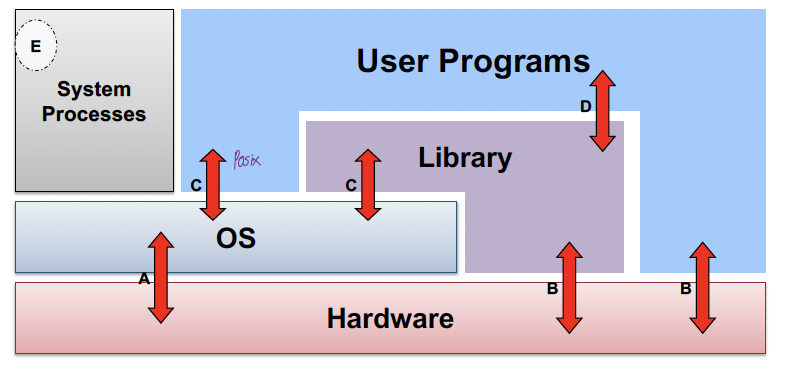
\includegraphics[width=0.9\linewidth]{01_general_os.png}
      \item \textbf{Monolithic OS}: Kernel == 1 big program, (+) good performance (-) highly coupled components, complicated internal structure, eg. Most Unix variants, Windows
      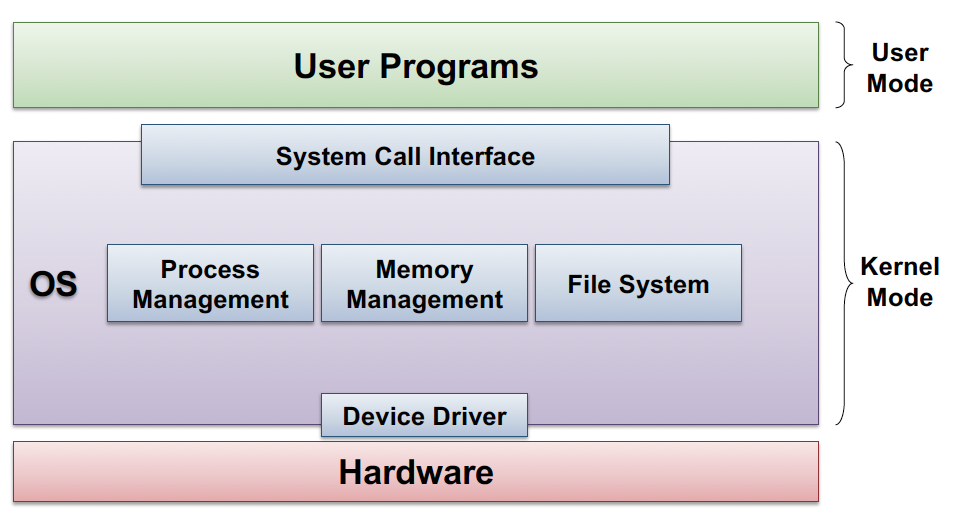
\includegraphics[width=0.9\linewidth]{02_monolithic_os.png}
      \item \textbf{Microkernel OS}: Kernel is small, provides basic \& essential facilities, uses IPC to communicate, (+) More modular, robust, better isolation, protection between kernel \& user spaces (-) lower performance
      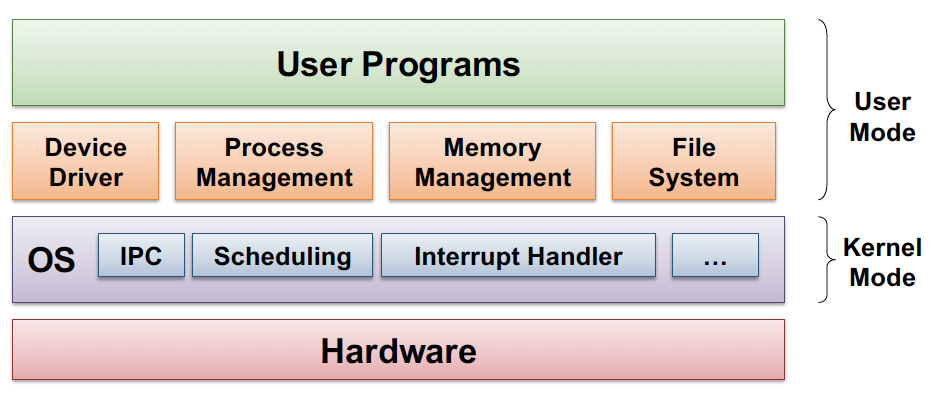
\includegraphics[width=0.9\linewidth]{03_microkernel_os.png}
      \item \textbf{Layered Systems OS:} Generalisation of Monolithic system, hierarchy of layers where upper layers make use of lower layers $\rightarrow$ Lowest layer is hardware, Highest layer is user interface
      \item \textbf{Client-Server Model:} Variation of Microkernel where server process is built on top of microkernel, client \& server process can be on separate machine
    \end{itemize}

    \subsection{Virtual Machines}
    \begin{itemize}
      \item \textbf{Definition:} Software emulation of hardware, normal OS then run on top of VM (aka. Hypervisor)
      \item \textbf{Type 1 Hypervisor:} Runs directly on hardware (more efficient), provides individual VMs to guest OSes
      \item \textbf{Type 2 Hypervisor:} Runs on host OS (more overhead), guest OS runs inside VM (more common for normal users)
    \end{itemize}

    \section{Process Abstraction}
    \subsection{Introduction to Process Abstraction}
    \begin{itemize}
      \item \textbf{Process Definition:} Abstraction to describe a running program
      \item \textbf{Process Abstraction Definition:} Dynamic abstraction for executing program (using data structure to represent information required to describe a running program); Consists of
      \begin{enumerate}
        \item Memory Context (code, data)
        \item Hardware Context (registers, program counter)
        \item OS Context (process properties, resources used)
      \end{enumerate}
    \end{itemize}

    \subsection{Memory Context}
    \subsubsection{Stack Memory}
    \begin{itemize}
      \item \textbf{Stack Memory Region:} Memory region to store information regarding function invocation (described by a stack frame)
      \item \textbf{Stack Frame:} Contains Return address of Caller, Parameters for function, Local variables, other information; Different ways to set up stack frame
      \item \textbf{Stack Pointer:} Indicates top of stack region
      \item \textbf{Frame Pointer:} Points to a fixed location in stack frame, other items are accessed as displacement from fboxsep
      \item \textbf{Saved Registers:} No. of General Purpose Registers (GPRs) are limited $\rightarrow$ memory can temporarily hold GPR value when GPRs are exhausted so that GPRs can be used for other purposes $\rightarrow$ GPR value can be restored afterwards 
      \item \textbf{Stack Frame Illustration:}
      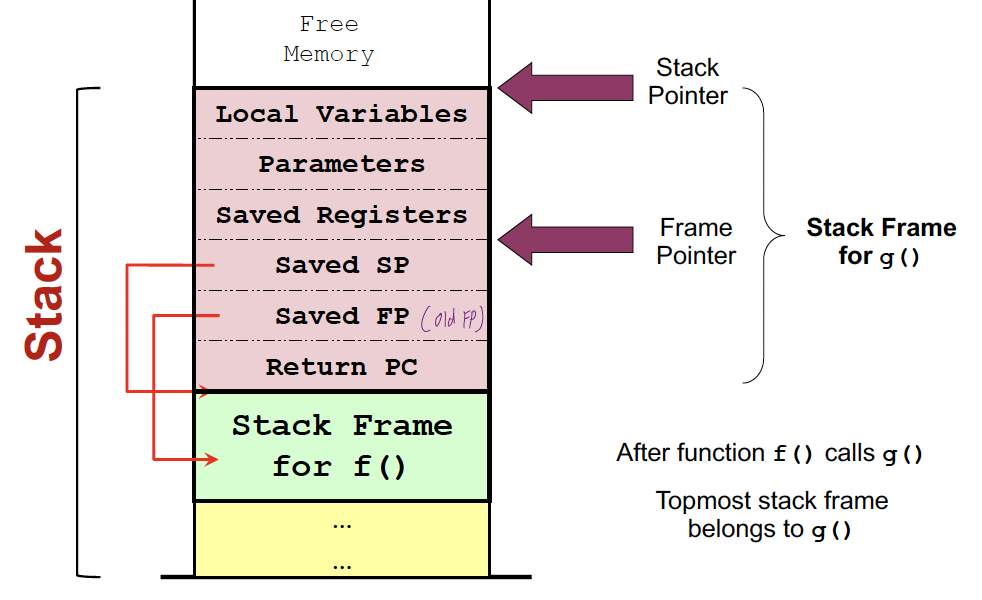
\includegraphics[width=0.9\linewidth]{04_stack_frame.png}
      \begin{enumerate}
        \item \underline{Executing function call:} Caller passes parameters with registers \& saves Return PC on stack $\rightarrow$ transfers control to callee $\rightarrow$ Callee saves registers used by it, saves old FP \& SP, allocates space for local variables of callee, adjusts SP to point to new stack top
        \item \underline{Returning from function call:} Callee restores saved registers, FP \& SP $\rightarrow$ Transfers control to caller using saved Return PC
      \end{enumerate}
    \end{itemize}

    \subsubsection{Heap Memory}
    \begin{itemize}
      \item \textbf{Dynamically allocated memory:} Acquire memory space during execution time; Cannot be placed in data region as memory is allocated at runtime only, size is not known during compilation; Cannot be placed in stack region as deallocation time is not definite
    \end{itemize}

    \subsection{OS Context}
    \begin{itemize}
      \item \textbf{Process ID:} Unique among processes, distinguishes processes from each other
      \item \textbf{Process Model:} Set of states \& transitions of a process
      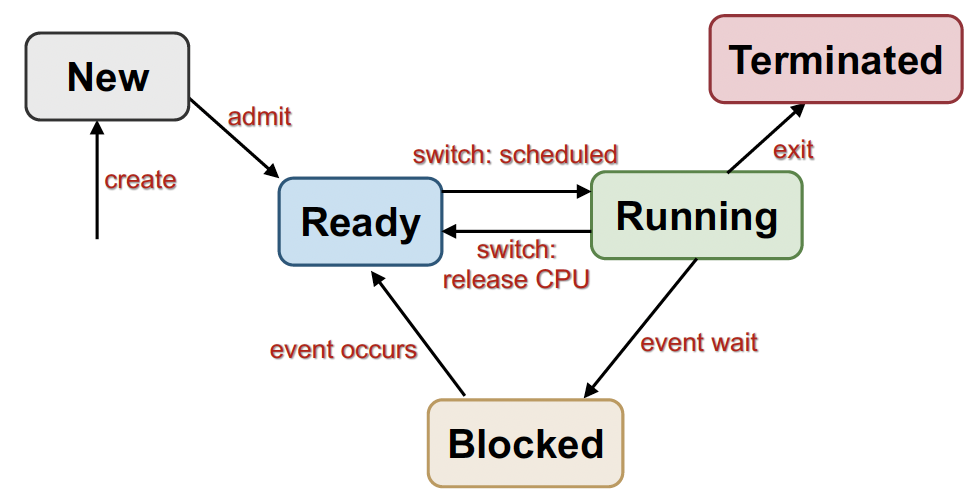
\includegraphics[width=0.9\linewidth]{05_process_model.png}
      \begin{enumerate}
        \item New: New process created, not yet ready
        \item Ready: Process waiting to run
        \item Running: Process being executed on CPU
        \item Blocked: Process waiting for event (eg. system call, waiting for I/O)
        \item Terminated: Process has finished execution
      \end{enumerate}
      \item \textbf{Process Table \& Process Control Block:} PCB stores entire execution context for a process (Hardware: PC, FP, SP, GPRs; Memory: Text, Data, Heap, Stack; OS: PID, Process State) $\rightarrow$ Kernel maintains PCBs for all processes in 1 table
    \end{itemize}

    \subsection{System Calls}
    \begin{itemize}
      \item \textbf{Definition of System Call:} API to OS (Provides way of calling services within Kernel, NOT same as normal function call)
      \item \textbf{Function Wrapper:} Library version that has same name \& parameters as system call (eg. \lstinline|getPid()| is library call that has same name as system call)
      \item \textbf{Function Adapter:} Library version has less parameters, more flexible parameter values compared to system call (eg. \lstinline|printf()| is library call that makes \lstinline|write()| system call)
      \item \textbf{System Call Mechanism:}
      \begin{enumerate}
        \item User program invokes library call via normal function call
        \item Library call places system call number in a register
        \item Library call executes TRAP to switch from user mode to kernel mode
        \item In kernel mode, system call handler is determined (handled by dispatcher)
        \item System call handler is executed
        \item System call handler ends, control returns to library call (switch from kernel mode to user mode)
        \item Library call returns to user program via normal function return
      \end{enumerate}
    \end{itemize}

    \subsection{Exceptions \& Interrupts}
    \begin{itemize}
      \item \textbf{Exceptions:} Caused by machine level instructions, synchronous (fixed point in program execution), executes exception handler
      \item \textbf{Interrupts:} Caused by external events, asynchronous (any point in program execution), executes interrupt handler
      \item \textbf{Handler Routine:} Save register/CPU state $\rightarrow$ Perform handler routine $\rightarrow$ Restore register/CPU $\rightarrow$ Return from interrupt
    \end{itemize}
\end{multicols*}
\end{document}
